\documentclass[oneside, 11pt]{article}

\usepackage[T1]{fontenc}
\usepackage[utf8]{inputenc}
\usepackage[english]{babel}

\usepackage{fouriernc}
\usepackage[detect-all, binary-units, separate-uncertainty=true,
            per-mode=symbol, retain-explicit-plus, retain-unity-mantissa=false]{siunitx}

\usepackage{setspace}
\setstretch{1.2}

\setlength{\parskip}{\smallskipamount}
\setlength{\parindent}{0pt}

\usepackage[headheight=14pt]{geometry}
\geometry{marginparwidth=0.5cm, verbose, a4paper, tmargin=3cm, bmargin=3cm,
          lmargin=2cm, rmargin=2cm}

\usepackage{float}

\usepackage[fleqn]{amsmath}
\numberwithin{equation}{section}
\numberwithin{figure}{section}

\usepackage{graphicx}
\graphicspath{{images/}{../../../images/}}

\usepackage{tikz}
\usetikzlibrary{shapes}
\usetikzlibrary{plotmarks}

\newcounter{Exercise}
\setcounter{Exercise}{1}
\usepackage{xcolor}
\definecolor{shadecolor}{gray}{0.9}
\usepackage{framed}
\usepackage{caption}

\usepackage{url}


\usepackage{fancyhdr}
\pagestyle{fancy}
\fancyhf{}
\rhead{\thepage}
\renewcommand{\footrulewidth}{0pt}
\renewcommand{\headrulewidth}{0pt}

\fancypagestyle{firststyle}
{
    \fancyhf{}
    \rhead{\thepage}
    \cfoot{
\includegraphics[height=30pt]{HiSPARClogo}}
    \rfoot{
\includegraphics[height=25pt]{CCbysa}}
    \lfoot{
\includegraphics[height=30pt]{NIKHEFlogo}}
    \renewcommand{\footskip}{50pt}
    \renewcommand{\footrulewidth}{0.1pt}
    \renewcommand{\headrulewidth}{0pt}
}

\newcommand{\figref}[1]{Figuur~\ref{#1}}

\newcommand{\hisparc}{\textsmaller{HiSPARC}\xspace}
\newcommand{\kascade}{\textsmaller{KASCADE}\xspace}
\newcommand{\sapphire}{\textsmaller{SAPPHiRE}\xspace}
\newcommand{\jsparc}{\textsmaller{jSparc}\xspace}
\newcommand{\hdf}{\textsmaller{HDF5}\xspace}
\newcommand{\aires}{\textsmaller{AIRES}\xspace}
\newcommand{\csv}{\textsmaller{CSV}\xspace}
\newcommand{\python}{\textsmaller{PYTHON}\xspace}
\newcommand{\corsika}{\textsmaller{CORSIKA}\xspace}
\newcommand{\labview}{\textsmaller{LabVIEW}\xspace}
\newcommand{\daq}{\textsmaller{DAQ}\xspace}
\newcommand{\adc}{\textsmaller{ADC}\xspace}
\newcommand{\hi}{\textsc{h i}\xspace}
\newcommand{\hii}{\textsc{h ii}\xspace}
\newcommand{\mip}{\textsmaller{MIP}\xspace}
\newcommand{\hisparcii}{\textsmaller{HiSPARC II}\xspace}
\newcommand{\hisparciii}{\textsmaller{HiSPARC III}\xspace}

\DeclareSIUnit{\electronvolt}{\ensuremath{\mathrm{e\!\!\:V}}}

\DeclareSIUnit{\unitsigma}{\ensuremath{\sigma}}
\DeclareSIUnit{\mip}{\textsmaller{MIP}}
\DeclareSIUnit{\adc}{\textsmaller{ADC}}

\DeclareSIUnit{\gauss}{G}
\DeclareSIUnit{\parsec}{pc}
\DeclareSIUnit{\year}{yr}



\begin{document}

\title{Telescopen}
\author{N.G. Schultheiss}
\date{}

\maketitle
\thispagestyle{firststyle}

\section{Inleiding}

Deze module volgt op de module ``Lenzen'' of ``Lenzen slijpen''.
Deze module wordt vervolgd met de module ``Telescopen gebruiken''.
Je kunt met na deze module een telescoop bouwen en de werking verklaren.

In de vorige modules is kennis gemaakt met lenzen en spiegels.


\section{Soorten telescopen}

Telescopen vallen uiteen in twee groepen, de refractors en de reflectors.
Bij een refractor valt het licht eerst op een lens. Bij een reflector
valt het licht eerst op een spiegel. Dit eerste optische element wordt
ook wel het objectief genoemd. Het objectief zit het dichtst object
(voorwerp) dat men bekijkt. Het optisch element dat het dichtst bij
het oog (oculus) zit, noemt men het oculair.

De telescoop die door Galileo Galileï tijdens de renaisance werd gebruikt
was een refractor. Deze telescoop had een speciale constructie, met
een bol objectief en een hol oculair, en wordt ook wel de hollandse
kijker genoemd. 


\paragraph*{Opdracht 1:}

\emph{Leg uit dat het beeld van de hollandse kijker rechtop staat.}

\begin{figure}[H]
\noindent \begin{centering}
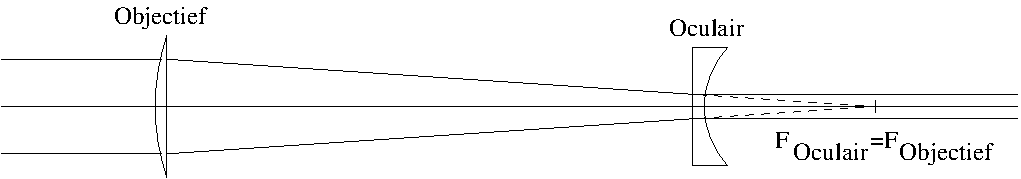
\includegraphics[scale=0.75]{hollandseKijker}
\par\end{centering}

\caption{De hollandse kijker}
\end{figure}


De hollandse kijker werd in de $17^{e}$ eeuw verbeterd door Christiaan
Huygens met een nieuw soort oculair. Dit oculair bestaat uit twee
lenzen, samen werken deze als één lens. Dit nieuwe oculair is in de
$18^{e}$ eeuw nog eens door Jesse Ramsden aangepast.


\paragraph*{Opdracht 2:}

\emph{Leg uit dat het beeld in een Huygens objectief op zijn kop staat.}


\paragraph*{Opdracht 3:}

\emph{Leg uit wat het verschil tussen een Huygens objectief en een
Ramsden objectief is.}

\begin{figure}[H]
\noindent \begin{centering}
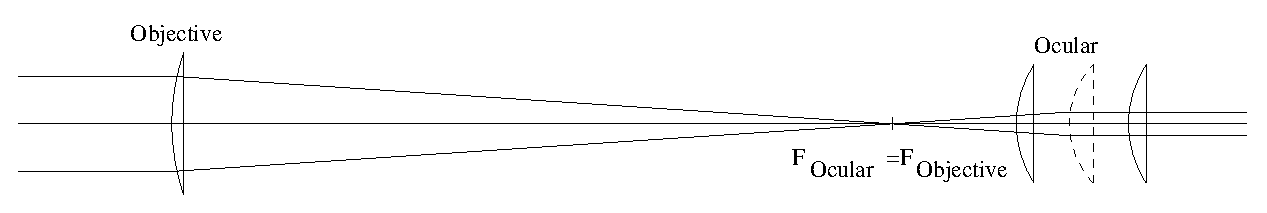
\includegraphics[scale=0.75]{huygens}
\par\end{centering}

\caption{Een telescoop met een Huygens oculair}
\end{figure}


Isaac Newton, een tijdgenoot van Huygens, gebruikte een spiegel in
plaats van een lens als objectief. Dit is de eerste refractor. Bij
de spiegel vallen het brandpunt van de spiegel en het oculair samen.
Deze brandpunten moeten wel samenvallen, dit hoeft echter niet precies
op de vlakke spiegel.

\begin{figure}[H]
\noindent \begin{centering}
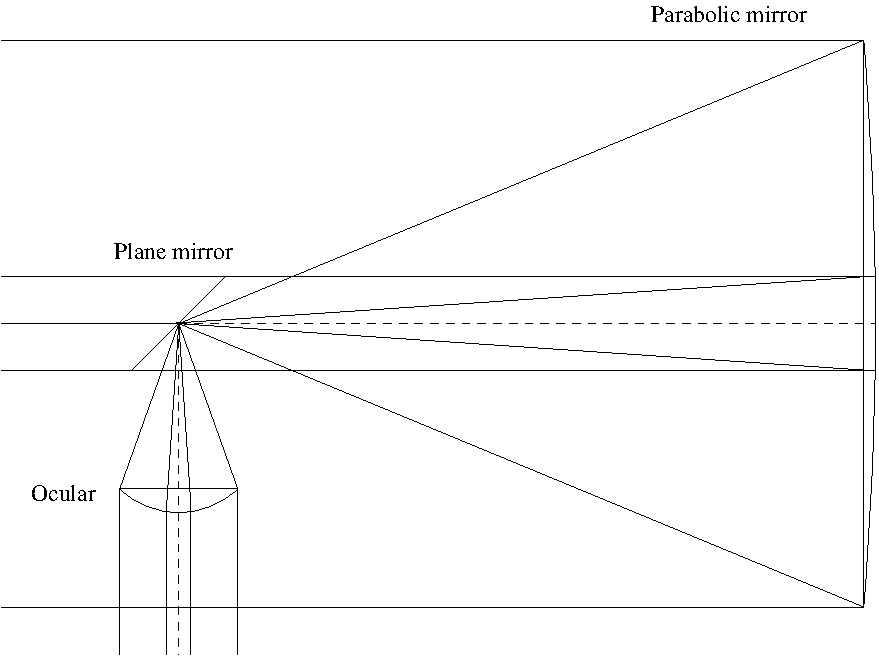
\includegraphics[scale=0.75]{newton}
\par\end{centering}

\caption{De Newton refractor}
\end{figure}



\paragraph*{Opdracht 4:}

\emph{Een grote telescoop is altijd een reflector en nooit een refractor.
Verklaar waarom dit zo is.}

Eind $17^{e}$ eeuw / begin $18^{e}$ eeuw gebruikte Friedrich Wilhelm
Herschel achtereenvolgens steeds grotere refractors om het zonnestelsel
en de sterren te bestuderen. Hij kwam op het idee dat het zonnestelsel
deel uitmaakte van het melkwegstelsel. Zijn zus Caroline Lucretia
Herschel heeft deze telescopen ook gebruikt om de asteroïden te bestuderen.
Zijn zoon John Frederick William Herschel zette hun werk voort en
experimenteerde daarnaast ook met fotografisch materiaal.


\section{Rekenen aan een telescoop}


\subsection{De vergroting}

Een aantal eigenschappen van een telescoop is uit te rekenen. Een
eerste belangrijke eigenschap lijkt de vergroting van de telescoop.
Zoals uit figuur 2.1, 2.2 en 2.3 blijkt valt er een evenwijdige bundel
in het objectief en komt er een evenwijdige bundel uit het objectief.
De vergroting van de telescoop is dus anders dan de vergroting van
een lens. 

\begin{figure}[H]
\noindent \begin{centering}
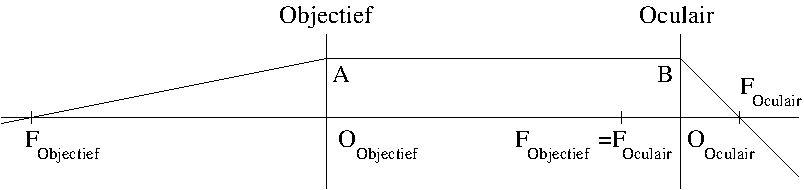
\includegraphics[scale=0.75]{schema}
\par\end{centering}

\caption{Schematische voorstelling van de telescoop}
\end{figure}


In figuur 3.1 zie je hoe het licht door een telescoop gaat. Als het
licht voor het objectief door het brandpunt gaat, gaat het licht in
de telescoop evenwijdig aan de hoofdas. Na het oculair gaat het licht
weer door het brandpunt. Bij het objectief (aan de invallende kant)
maakt het licht een hoek met de hoofdas: $\angle\mathrm{A}\mathrm{F_{objectief}O_{objectief}}$.
Na het objectief zien we de hoek tussen de hoofdas en de lichtstraal
als $\angle\mathrm{BF_{Oculair}O_{Oculair}}$.

\begin{equation}
\tan(\angle\mathrm{B}\mathrm{F_{Oculair}O_{Oculair}})
=\frac{\mathrm{B}\mathrm{O_{Oculair}}}{\mathrm{F_{Oculair}O_{Oculair}}}
\end{equation}


\begin{equation}
\tan(\angle\mathrm{A}\mathrm{F_{Objectief}O_{Objectief}})
=\frac{\mathrm{A}\mathrm{O_{Objectief}}}{\mathrm{F_{Objectief}O_{Objectief}}}
\end{equation}


Deze formules delen we op elkaar:

\begin{equation}
\frac{\tan(\angle\mathrm{B}\mathrm{F_{Oculair}O_{Oculair}})}{\tan(\angle\mathrm{A}\mathrm{F_{Objectief}O_{Objectief}})}
=\frac{\left(\frac{\mathrm{B}\mathrm{O_{Oculair}}}{\mathrm{F_{Oculair}O_{Oculair}}}\right)}{\left(\frac{\mathrm{A}\mathrm{O_{Objectief}}}{\mathrm{F_{Objectief}O_{Objectief}}}\right)}
\end{equation}


De twee lijnstukken $\mathrm{A}\mathrm{O_{Objectief}}$ en $\mathrm{B}\mathrm{O_{Oculair}}$
hebben dezelfde lengte:

\begin{equation}
\frac{\tan(\angle\mathrm{B}\mathrm{F_{Oculair}O_{Oculair}})}{\tan(\angle\mathrm{A}\mathrm{F_{Objectief}O_{Objectief}})}
=\frac{\mathrm{F_{Objectief}O_{Objectief}}}{\mathrm{F_{Oculair}O_{Oculair}}}
\end{equation}


Voor kleine hoeken geldt dat de tangens van de hoek gelijk is aan
de hoek in radialen:
\begin{equation}
\frac{\angle\mathrm{B}\mathrm{F_{Oculair}O_{Oculair}}}{\angle\mathrm{A}\mathrm{F_{Objectief}O_{Objectief}}}
=\frac{\mathrm{\mathit{f}_{Objectief}}}{\mathrm{\mathit{f}_{Oculair}}}
\end{equation}


\begin{equation}
Hoekvergroting=\frac{\mathrm{\mathit{f}_{Objectief}}}{\mathrm{\mathit{f}_{Oculair}}}
\end{equation}



\paragraph*{Opdracht 4:}

\emph{Christiaan Huygens bouwde telescopen. Hij ontdekte Titan met een
telescoop met $f_{\mathrm{objectief}}=12[\mathrm{voet}]$ en
$f_{\mathrm{oculair}}=3[\mathrm{duim}]$. Bereken de vergroting van de
telescoop waarmee hij Titan ontdekte.}


\subsection{De resolutie}

De hoekvergroting is wel van enig belang. Als je de gegevens van telescopen
opzoekt, wordt deze vergroting echter zelden gegeven. Omdat de hoekvergroting
ook van de sterkte van het oculair afhangt, is deze eenvoudig aan
te passen.

De diameter wordt veel belangrijker gevonden. Het blijkt dat de diameter
van de telescoop direct te koppelen is aan de resolutie of de nauwkeurigheid
waarmee je met een telescoop hemelobjecten kan waarnemen. Als twee
sterren dicht bij elkaar staan, of als een planeet rond een ster draait,
komen de lichtstralen van de twee hemelobjecten bijna parallel bij
de telescoop aan. Als vuistregel kun je zeggen dat de twee lichtbundels
te scheiden zijn als ze boven en onder bij de spiegel meer dan een
golflengte verschillen.

\begin{figure}[H]
\noindent \begin{centering}
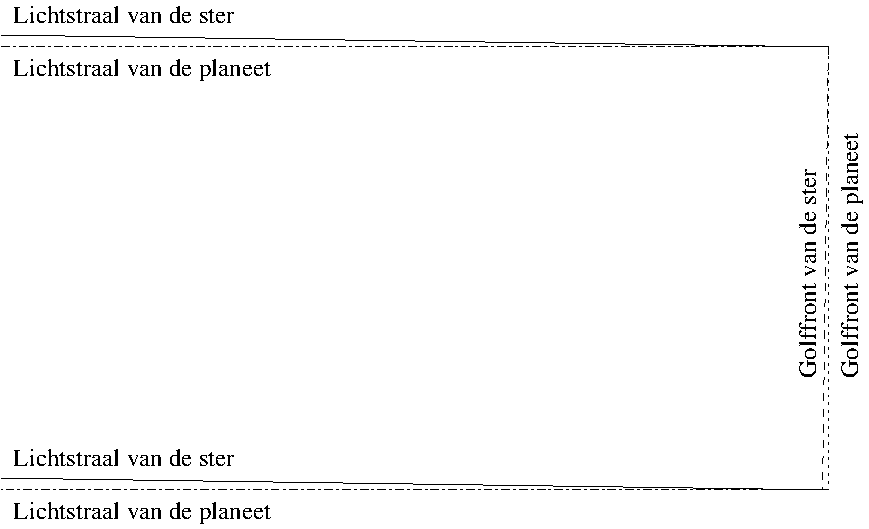
\includegraphics[scale=0.75]{resolutie}
\par\end{centering}

\caption{De resolutie van een telescoop}
\end{figure}


De kleinste hoek die met een telescoop te zien is, is met de sinus
of de tangens te berekenen:

\begin{equation}
\sin(\alpha)\approx \tan(\alpha)\approx\frac{\lambda}{Diameter}
\end{equation}


De hoek tussen een planeet en een ster is te berekenen met:

\begin{equation}
\alpha=\frac{afstand_{planeet,ster}}{afstand_{telescoop,ster}}
\end{equation}



\paragraph*{Opdracht 4:}

\emph{Een alien op $\varepsilon$ Eri, op een afstand van 10,522 lichtjaar,
bouwt een telescoop en kijkt daarmee naar de Zon. De alien ziet dat
rond de Zon een klein blauw planeetje draait. Zoek op wat de afstand
van de Aarde tot de Zon is. Zoek op wat de golflengte van blauw licht
is. Bereken de diameter van de telescoop van de alien.}


\paragraph*{Opdracht 5:}

\emph{Leg uit of Mars, de rode planeet, moeilijker of makkelijker
door de alien waar te nemen is.}

In de praktijk heb je een grotere telescoop nodig omdat een ster veel
meer licht geeft daan een planeet. De zon heeft eendiameter van 1392000km
en de Aarde heeft een diameter van 12742km. Dit is ongeveer 1000 maal
zo klein.


\paragraph*{Opdracht 6:}

\emph{Leg uit dat de Aarde als deze net zo veel licht per $m^{2}$
geeft 1000000 minder licht geeft dan de zon. In werkelijkheid geeft
de Aarde natuurlijk veel minder licht. Welke gevolgen heeft dit voor
de nauwkeurigheid van de meting en daarmee de grootte van de telescoop?}

\end{document}
